\documentclass[journal]{IEEEtran}
\usepackage[T1]{fontenc}
\usepackage[utf8]{inputenc}
\usepackage{amsmath,amssymb}
\usepackage{booktabs}
\usepackage{graphicx}
\usepackage{multirow}
\usepackage{microtype}
\usepackage{url}
\usepackage{xcolor}
\usepackage{array}
\usepackage{tabularx}
\usepackage{threeparttable}
\usepackage{siunitx}
\usepackage{balance}
\usepackage{hyperref}
\hypersetup{hidelinks}
\sisetup{detect-all,round-mode=places,round-precision=3}
\graphicspath{{figures/}}

\title{When More Motion Modeling Hurts: Causal Latency Compensation for Streaming Object Detection}

\author{Antonio Pereira Jr.\\
\small Faculdade de Engenharia El\'etrica e Biom\'edica, Instituto de Tecnologia, Universidade Federal do Par\'a, Bel\'em, Brazil\\
\small Corresponding author: \texttt{apereira@ufpa.br}
\thanks{Repository URL, release tag, and archival DOI must be inserted before submission.}}

\begin{document}
\maketitle

\begin{abstract}
A detector output computed from an image at time $t$ is applied at $t+\Delta$, after both the camera and scene objects have moved. We compared ego-motion-only propagation (B3) with B3 plus an uncertainty-damped causal object-motion estimate (B5) on a frozen Argoverse~2 cohort of 80 development, 20 model-selection, and 50 held-out logs, using prespecified parameters and a 300-ms high-yaw primary endpoint. B5 increased normalized center error relative to B3 by 19.18\% for YOLO11n, 21.06\% for YOLO11s, and 16.60\% for RT-DETR-L; paired bootstrap intervals excluded zero. B3 also outperformed stale boxes, constant image velocity, SORT, ByteTrack, and OC-SORT predictions. Full-frame AP75, recall, and false positives supported the localization result, whereas paired AP50:95 differences were inconclusive. Oracle future displacement improved on B3, showing that object motion is useful in principle, but causal velocity-sign and association errors dominated the deployed estimate. The B5 disadvantage increased from 2.58\% at 100~ms to 30.40\% at 500~ms, and a frozen causal gate selected B5 in no eligible extension comparisons. Measured ego-motion propagation is therefore the safer default for this system; object-motion augmentation should be enabled only by a reliability criterion validated on untouched data.
\end{abstract}


\begin{IEEEkeywords}
autonomous driving, streaming perception, object detection, ego-motion compensation, multi-object tracking, latency compensation, Argoverse~2, RT-DETR.
\end{IEEEkeywords}

\section{Introduction}
\IEEEPARstart{O}{bject} detectors are usually evaluated as if the scene stood still during inference. In an embodied system, a result computed from an image acquired at time $t$ becomes actionable at $t+\Delta$, after both the camera and scene objects have moved. Streaming-perception benchmarks have formalized this mismatch and shown that offline accuracy overstates online performance \cite{Li2020Streaming,Yang2022Streaming,Wang2023ASAP}. This leaves a practical post-processing problem: transporting a delayed detector box into the camera frame that exists when the result arrives.

Image-space trackers extrapolate detections with constant-velocity or Kalman models \cite{Kalman1960,Bewley2016SORT}; ByteTrack and OC-SORT add broader association and observation-centric updates \cite{Zhang2022ByteTrack,Cao2023OCSORT}. On an ego-moving platform, camera motion contributes a second displacement component, motivating pose-aware propagation that combines depth, ego motion, and target dynamics \cite{Mahdian2024EMAP}. The expected hierarchy is clear: correcting both ego and object motion should beat correcting ego motion alone.

An initial feasibility analysis on a small nuScenes subset suggested that object-motion augmentation could improve latency compensation when privileged instance-linked histories were available. We subsequently froze the modeling choices and evaluated both methods under common, deployable information constraints on Argoverse 2. Under this evaluation, the apparent benefit reversed. The present study reports the frozen held-out comparison and the diagnostic analyses used to localize that reversal. Here we ask whether it survives a transformer-based end-to-end detector, whether ego-only propagation is competitive with established causal tracker predictions, and whether full-frame current-time metrics agree with the matched-object result.

This paper makes five contributions: a prespecified B3-versus-B5 reversal replicated across YOLO11n, YOLO11s, and RT-DETR-L \cite{Zhao2024RTDETR}; a comparison of both geometric models against stale, constant-velocity, SORT, ByteTrack, and OC-SORT baselines; separate persistent-object and full-frame target-time evaluations; failure localization through oracle substitutions and fixed diagnostic categories; and a one-shot evaluation of an untouched causal gate. Oracle displacement confirmed that object motion contains useful corrective information, while universal application of its noisy causal estimate increased error.

\section{Related Work}
\subsection{Latency-aware perception}
Streaming accuracy evaluates a perception stack at the time its output becomes available rather than at image acquisition \cite{Li2020Streaming}. Later work forecast future-frame detections and benchmarked complete vision-centric streaming systems \cite{Yang2022Streaming,Wang2023ASAP}. Our analysis targets a narrower deployment layer: transporting fixed detector boxes through a known latency without retraining the detector.

\subsection{Tracking-by-detection and motion prediction}
SORT uses a constant-velocity Kalman filter with Hungarian assignment \cite{Bewley2016SORT,Kuhn1955}. ByteTrack associates both high- and low-confidence detections to preserve trajectories \cite{Zhang2022ByteTrack}. OC-SORT applies observation-centric velocity updates to limit error accumulation after missed observations \cite{Cao2023OCSORT}. These trackers provide stronger causal comparators than a stale box or a two-frame velocity estimate, and they expose the central uncertainty asymmetry of the problem: ego motion is shared across a frame and measured from platform poses, whereas object motion depends on object-specific association, depth, and detector stability over time.

\subsection{Autonomous-driving datasets and detectors}
AV2 provides synchronized cameras, lidar, ego poses, calibration, and tracked annotations \cite{Wilson2021AV2}. nuScenes served only for secondary harmonization \cite{Caesar2020nuScenes}. YOLO11n and YOLO11s supplied two detector capacities through the Ultralytics implementation \cite{Ultralytics2024}; RT-DETR-L supplied an end-to-end transformer detector without non-maximum suppression as an architecture-level robustness test \cite{Zhao2024RTDETR}.

\section{Problem Formulation}
Let $b_t$ be a detector box computed from an image acquired at time $t$ and delivered after latency $\Delta$. The target is the box geometry at $t+\Delta$. B3 back-projects the source box through source-time depth, transforms it with measured ego poses, and reprojects it into the target camera. B5 adds an uncertainty-damped estimate of object displacement obtained causally from associated detector history.

For detector $d$ and log $l$, the primary error is the normalized center distance
\begin{equation}
 e_{l,d}=\frac{\sqrt{(\hat c_x-c_x)^2+(\hat c_y-c_y)^2}}
 {\sqrt{W^2+H^2}},
\end{equation}
where $(W,H)$ is image size. The primary estimand is the median across logs of the paired within-log relative difference
\begin{equation}
 r_l=\frac{\widetilde e_{l,\mathrm{B5}}-\widetilde e_{l,\mathrm{B3}}}
 {\widetilde e_{l,\mathrm{B3}}}.
\end{equation}
Positive values indicate harm from object-motion augmentation.

\section{Materials and Methods}
\subsection{Frozen cohorts and detector outputs}

Before evaluating the held-out logs, we fixed the cohort-selection seed, modeling parameters, analysis definitions, and the 300-ms high-yaw primary endpoint. Table~\ref{tab:params} records these frozen choices.

The fixed AV2 cohort contained 80 development, 20 model-selection, and 50 held-out validation logs, selected before outcome analysis with seed 20260717 using pre-outcome city, ego-speed, yaw, and traffic-density metadata. Only the forward ring camera, lidar, calibration, poses, and annotations were required.

All detectors ran at 640-pixel inference size and confidence threshold 0.25. RT-DETR-L used the \texttt{rtdetr-l.pt} checkpoint distributed through the Ultralytics framework; SHA-256 hashes of all three detector checkpoints are recorded in the repository manifest. The RT-DETR-L held-out run comprised 50 logs and 16,022 frames. Detector outputs were checkpointed before propagation. COCO detections were mapped to vehicle, pedestrian/cyclist, and other groups.

Latency horizons were 100, 200, 300, 400, and 500~ms. The frozen primary endpoint was 300~ms in the upper development-cohort quartile of absolute yaw rate (0.0170~rad/s). Forty held-out logs contained eligible matched comparisons at this endpoint for all three detectors; all 50 contributed to all-yaw analyses.

\subsection{Causal propagation and tracker baselines}
Seven methods were evaluated on identical eligible comparisons:
\begin{itemize}
\item T0: stale source box;
\item T1: constant image-space velocity;
\item T2: SORT Kalman prediction;
\item T3: ByteTrack causal prediction;
\item T4: OC-SORT causal prediction;
\item T5/B3: measured ego-motion-only propagation;
\item T6/B5: B3 plus uncertainty-damped estimated object motion.
\end{itemize}
Deployable methods saw only source-time detections and histories: no target-time detections, future annotation geometry, future identity, or future velocity entered their predictions.

B3 used source-box lidar depth, source and target ego poses, and calibrated camera projection. B5 estimated object velocity from same-class associated detector histories over at most 600~ms and four observations, multiplied object displacement by a frozen reliability weight based on lidar support, depth dispersion, and track age, and capped speed at 30~m/s. Table~\ref{tab:params} lists all frozen modeling and analysis parameters; they were fixed with the method specification before any AV2 outcome was computed and were not retuned afterward.

\begin{table}[t]
\caption{Frozen Modeling and Analysis Parameters}
\label{tab:params}
\centering
\footnotesize
\begin{threeparttable}
\begin{tabular}{@{}ll@{}}
\toprule
Parameter & Value \\
\midrule
\multicolumn{2}{@{}l}{\textbf{Cohorts and endpoint}} \\
Cohort selection seed & 20260717 \\
Development / model-sel.\ / held-out logs & 80 / 20 / 50 \\
Extension logs (gate; freeze seed 20260719) & 45 \\
Latency horizons & 100--500~ms, step 100 \\
Primary endpoint & 300~ms, high yaw \\
High-yaw threshold\tnote{a} & $|\dot\psi|\ge 0.0170$~rad/s \\
\midrule
\multicolumn{2}{@{}l}{\textbf{Detector inference}} \\
Input resolution & 640~px \\
Confidence threshold & 0.25 \\
Class mapping & vehicle, ped./cyclist, other \\
\midrule
\multicolumn{2}{@{}l}{\textbf{History association (B5)}} \\
Assignment & Hungarian, same class only \\
Minimum IoU & 0.10 \\
Max.\ normalized center distance & 0.15 \\
Maximum track gap & 600~ms \\
History length & 4 observations \\
\midrule
\multicolumn{2}{@{}l}{\textbf{Object-motion estimate (B5)}} \\
Motion model & const.\ velocity, 3-D history \\
$\alpha$--$\beta$ smoothing & $\alpha=0.65$ \\
Speed cap & 30~m/s \\
\midrule
\multicolumn{2}{@{}l}{\textbf{Reliability damping (B5)}} \\
Lidar-support saturation & 10 points \\
Depth-dispersion scale & 5.0~m \\
Track-age saturation & 3 observations \\
\midrule
\multicolumn{2}{@{}l}{\textbf{Depth recovery}} \\
Source & source-time lidar inside box \\
Statistic / uncertainty & median / scaled MAD \\
Minimum points; fallback & 1; box-geometry regression \\
\midrule
\multicolumn{2}{@{}l}{\textbf{Statistics}} \\
Independent unit & complete log \\
Bootstrap & 10{,}000 paired log-cluster repl. \\
Matched-object recall threshold & IoU 0.5 \\
\midrule
\multicolumn{2}{@{}l}{\textbf{Frozen causal gate}} \\
Model & $\ell_2$ logistic regr.\ ($C=1.0$) \\
Features & 13 causal source-time features \\
Decision threshold & 0.60 (grid 0.50--0.90)\tnote{b} \\
\bottomrule
\end{tabular}
\begin{tablenotes}
\item[a] Upper quartile of absolute yaw rate in the development cohort.
\item[b] Selected on model-selection logs under a 2-percentage-point recall-loss constraint; frozen before extension outcomes.
\end{tablenotes}
\end{threeparttable}
\end{table}

\subsection{Persistent-object and full-frame evaluation}
Matched-object analysis evaluated objects visible at both source and target times, reporting normalized center error, IoU, and recall at IoU 0.5. Full-frame evaluation compared all propagated detections with all target-time annotations, reporting AP50:95, AP50, AP75, precision, recall, false positives per frame, new-object miss fraction, and disappeared-object false-positive fraction. The scopes are reported separately because matched-object localization does not measure objects entering or leaving the frame during latency.

\subsection{Component substitutions and diagnostic mechanisms}
After the primary result was frozen, post hoc substitutions replaced one deployed component at a time with evaluation-only oracle information: association, historical boxes available no later than source time, historical three-dimensional positions, source depth, and future object displacement. The last substitution tests whether object motion can help in principle; it is nondeployable and was excluded from method-success decisions.

For objects harmed by B5, a fixed hierarchy assigned one of: incorrect association, velocity-sign error, velocity-direction error, velocity-magnitude error, detector-box jitter interpreted as motion, unstable short-track extrapolation, depth-induced projection error, missed acceleration, clipping/boundary error, distance-dependent failure, or unclassified. These labels are diagnostic and may reflect interacting causes.

\subsection{Sensitivity analysis and frozen causal gate}
Sensitivity analyses stratified results by latency, yaw, distance, detector confidence, track age, association confidence, velocity-sign consistency, class, and detector. Latency and detector strata were confirmatory; the rest were exploratory.

A previously frozen causal gate was evaluated once on available extension outputs. The gate used only source-time or causal-history features, was audited for leakage, and selected between B3 and B5 without threshold retuning. Success required lower center error than B3, noninferior IoU, at most two percentage points of recall loss, improvement in at least 70\% of extension logs, and a paired bootstrap interval excluding zero. RT-DETR prospective extension inference was incomplete and excluded.

\subsection{Statistics, runtime, and audits}
Logs were the independent units. Principal contrasts used paired absolute and relative differences, the percentage of logs improved, 10,000 paired log-cluster bootstrap replicates, and Wilcoxon signed-rank sensitivity tests. Full-frame AP was calculated both as pooled target-time detection performance and as paired log-level contrasts, with the aggregation level stated explicitly.

Audits checked detector identity, cohort overlap, timestamp order, complete T0--T6 model sets, duplicates, invalid coordinates, future-information flags, and independent headline recalculation. The final closure contained 100 valid current-detector scientific units plus four shard-summary rows, no duplicate or missing units, a provenance PASS, and a leakage PASS WITH LIMITATIONS reflecting incomplete extension coverage rather than leakage in the core held-out analysis. Twenty analysis-closure tests passed.

\section{Results}
\subsection{The reversal generalized across detector architectures}
At 300~ms in high-yaw driving, B5 increased normalized center error relative to B3 for all three detectors: 19.18\% for YOLO11n, 21.06\% for YOLO11s, and 16.60\% for RT-DETR-L (Table~\ref{tab:primary}; Fig.~\ref{fig:reversal}). All paired bootstrap intervals excluded zero, and B5 improved only 15.0\%, 20.0\%, and 17.5\% of eligible logs, respectively.

\begin{table*}[t]
\caption{Frozen 300-ms High-Yaw Held-Out Result}
\label{tab:primary}
\centering
\footnotesize
\begin{tabular}{@{}lrrr@{}}
\toprule
 & YOLO11n & YOLO11s & RT-DETR-L \\
\midrule
Eligible logs & 40 & 40 & 40 \\
Object comparisons & 11,425 & 14,089 & 25,729 \\
B3 normalized center error & 0.007003 & 0.005843 & 0.008512 \\
B5 normalized center error & 0.009146 & 0.007645 & 0.010176 \\
Paired B5 disadvantage & 19.18\% & 21.06\% & 16.60\% \\
95\% bootstrap interval & 10.80--37.05\% & 8.30--31.51\% & 11.93--23.38\% \\
B3 median IoU & 0.5550 & 0.5480 & 0.3647 \\
B5 median IoU & 0.5270 & 0.5026 & 0.3070 \\
Logs favoring B5 & 6/40 & 8/40 & 7/40 \\
Wilcoxon $p$ & 0.0016 & 0.0006 & 0.0010 \\
\bottomrule
\end{tabular}
\end{table*}

\begin{figure*}[t]
\centering
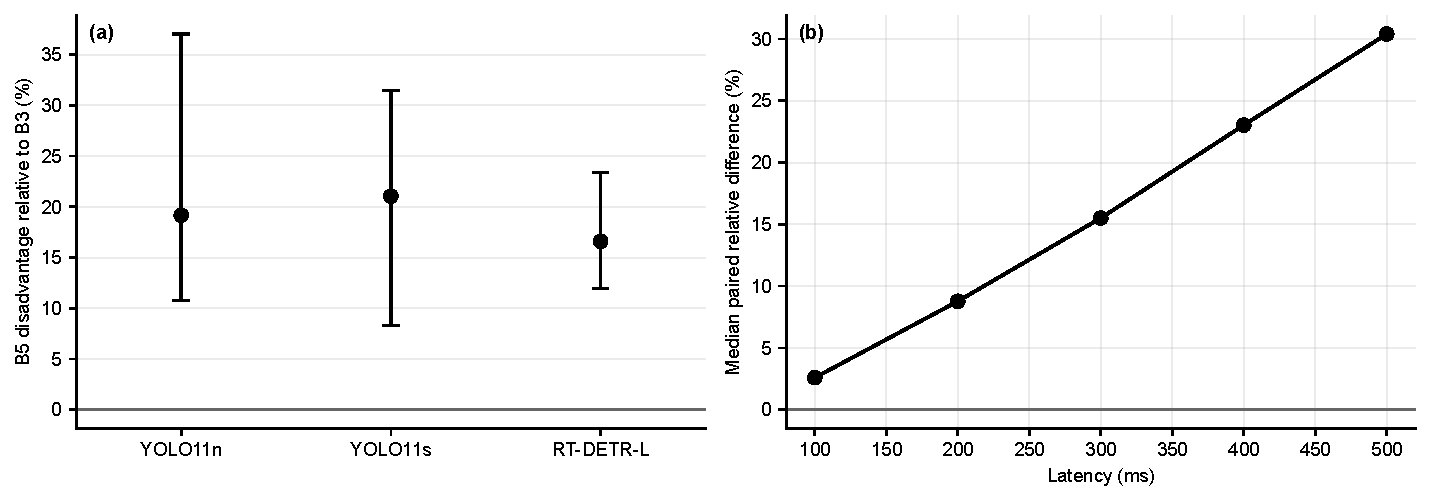
\includegraphics[width=0.92\textwidth]{figure2_reversal_latency.pdf}
\caption{Architecture and latency robustness. (a) Paired B5 disadvantage relative to B3 at the frozen 300-ms high-yaw endpoint; intervals are 10,000 paired log-cluster bootstrap intervals. (b) Median paired relative difference across all-yaw latency horizons.}
\label{fig:reversal}
\end{figure*}

In the all-yaw confirmatory analysis, harm grew monotonically with horizon: 2.58\% at 100~ms, 8.77\% at 200~ms, 15.50\% at 300~ms, 23.03\% at 400~ms, and 30.40\% at 500~ms---the signature of extrapolation error accumulating with time.

\subsection{B3 outperformed strong causal tracker predictions}
B3 had the lowest normalized center error among T0--T6 for every detector at the primary endpoint (Fig.~\ref{fig:trackers}). OC-SORT, the strongest alternative, remained 73.34\% worse than B3 for YOLO11n, 72.01\% for YOLO11s, and 56.23\% for RT-DETR-L, with paired bootstrap intervals excluding zero. Constant image velocity, SORT, and ByteTrack trailed further. These baselines were evaluated as causal box-prediction modules under identical delayed-detection conditions, not as complete tracking systems, so the comparison does not rank full MOT pipelines.

\begin{figure*}[t]
\centering
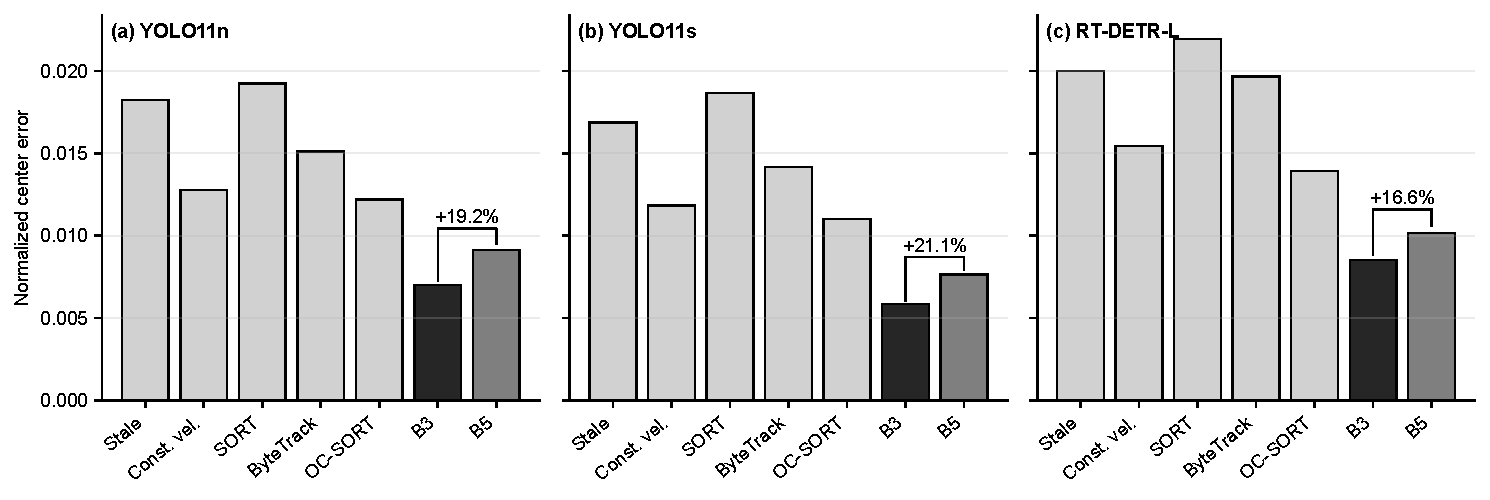
\includegraphics[width=0.98\textwidth]{figure1_tracker_architecture.pdf}
\caption{Causal baseline comparison at 300~ms in high-yaw held-out logs for (a) YOLO11n, (b) YOLO11s, and (c) RT-DETR-L. Bar heights are medians of within-log normalized center error; the two geometric models under comparison (B3, B5) are shaded darker than the causal baselines. The bracket links B3 and B5; its percentage is the paired log-level relative contrast, which differs from the ratio of the displayed aggregate medians.}
\label{fig:trackers}
\end{figure*}

\subsection{Full-frame evaluation supported localization but AP50:95 was mixed}
Full-frame evaluation agreed with the matched-object result where the two scopes overlap (Fig.~\ref{fig:fullframe}). At the frozen endpoint, B5 reduced AP75 by 20--28\% across detectors, reduced recall, and increased false positives per frame; paired log-level AP75 intervals excluded zero for both YOLO detectors and were borderline for RT-DETR-L. Paired AP50:95 intervals included zero for all three detectors, and pooled RT-DETR-L AP50:95 was nearly identical between methods (0.04661 for B3, 0.04685 for B5), showing how pooled and paired log-level aggregation can diverge.

\begin{figure*}[t]
\centering
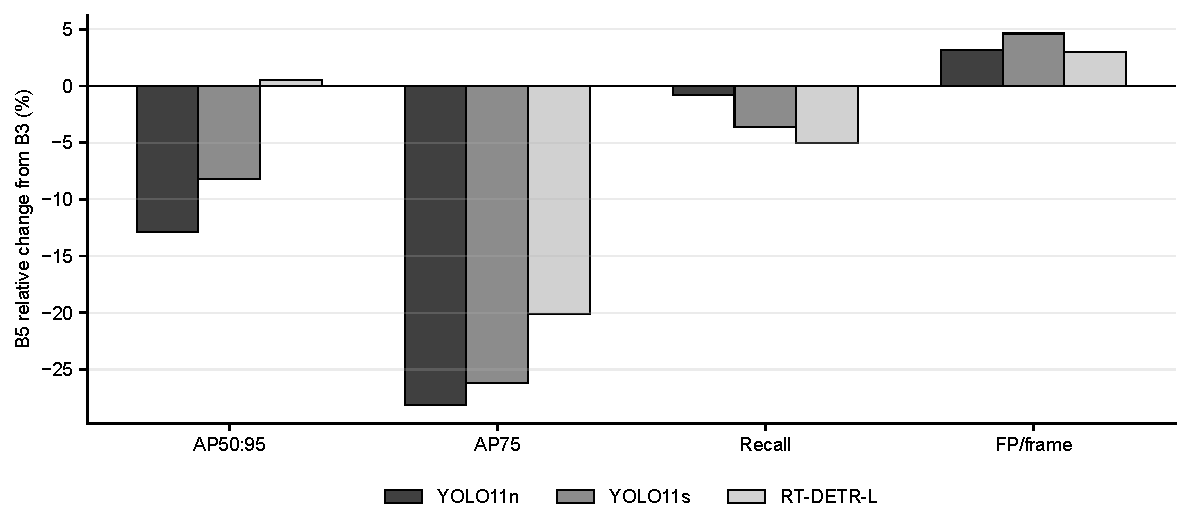
\includegraphics[width=0.88\textwidth]{figure5_full_frame.pdf}
\caption{Pooled full-frame current-time metrics at the frozen endpoint. Negative values for AP and recall favor B3 because B5 is lower; positive false positives per frame also favor B3. Paired log-level AP50:95 intervals included zero for all detectors.}
\label{fig:fullframe}
\end{figure*}

New-object miss fractions were high for both methods: objects entering the frame after the source time cannot be recovered by box propagation. This limitation is shared by all propagation-only methods and is why the two evaluation scopes are reported separately.

\subsection{Oracle substitutions showed useful signal obscured by estimation error}
Replacing deployed association with oracle identity reduced B5 error by 9.66\% for YOLO11n and 11.42\% for YOLO11s. Replacing detector-history boxes with true causal historical boxes removed a further 17.40\% and 18.77\%. Oracle future displacement improved on B3 by 11.11\% and 9.85\% (Fig.~\ref{fig:components}). Correct object displacement therefore helps in principle; the deployed estimator failed because its association and velocity errors exceeded the residual displacement it was correcting.

\begin{figure*}[t]
\centering
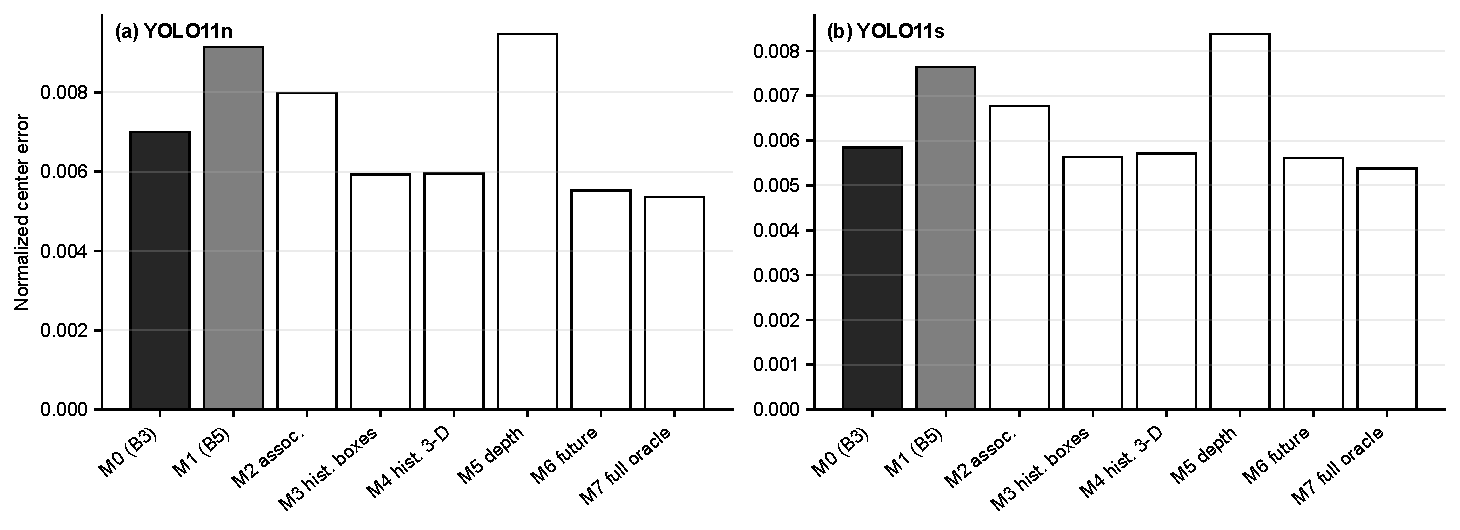
\includegraphics[width=0.92\textwidth]{figure3_component_substitution.pdf}
\caption{Component substitutions at 300~ms in high-yaw held-out logs for (a) YOLO11n and (b) YOLO11s. Filled bars are the deployed models (M0 is B3; M1 is B5). Open bars replace one component with oracle information: association (M2), historical boxes (M3), historical 3-D positions (M4), source depth (M5), future displacement (M6), and all components (M7). Future-displacement models are diagnostic and nondeployable.}
\label{fig:components}
\end{figure*}

\subsection{Failure mechanisms and exploratory operating strata}
Velocity-sign error was the leading mechanism, covering 37.16\% of harmed YOLO11n objects and 38.67\% of harmed YOLO11s objects, followed by incorrect association at 24.44\% and 22.79\%. Velocity-magnitude and direction errors each contributed 14--16\%; depth-induced projection errors were rare under the fixed hierarchy.

Harm was not uniform across operating conditions. For objects at 0--20~m, B5 reduced center error by 8.28\% and improved 69\% of logs; in the high-confidence detector stratum it reduced error by 15.76\% and improved 65\% of logs. Beyond 40~m it was 26.85\% worse, and 34.58\% worse at low confidence (Fig.~\ref{fig:mechanisms}). Selective compensation is plausible, but these strata are exploratory and do not validate the current selector.

\begin{figure*}[t]
\centering
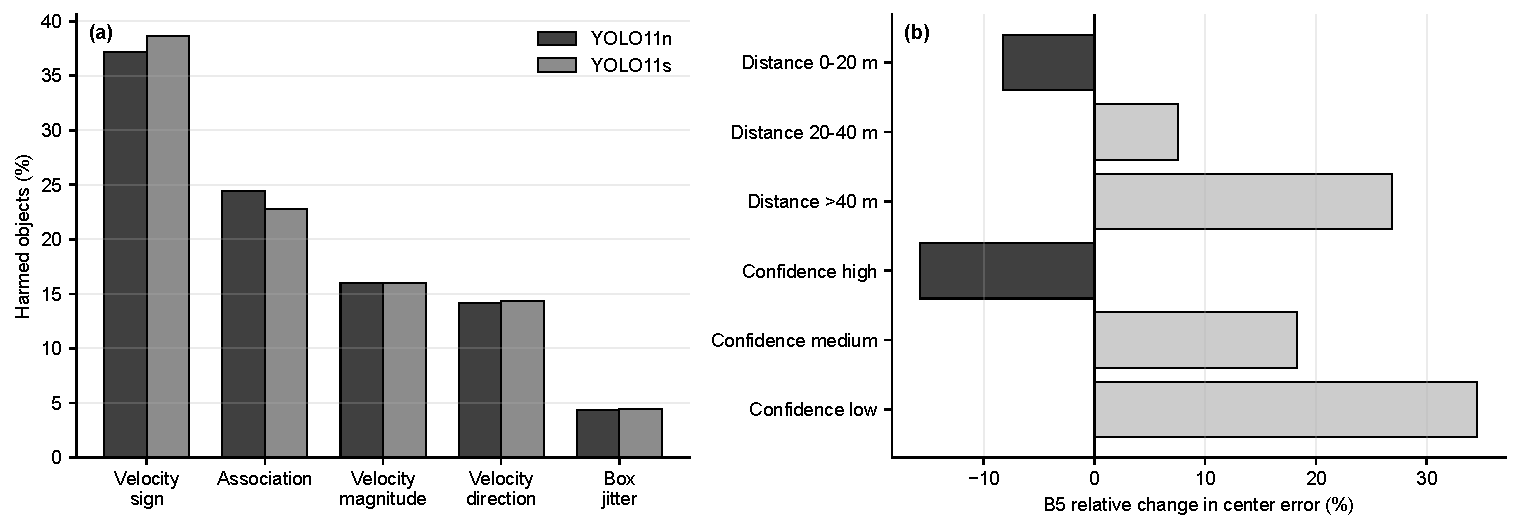
\includegraphics[width=0.96\textwidth]{figure4_failure_sensitivity.pdf}
\caption{Diagnostic mechanisms and exploratory operating strata. (a) Fixed hierarchical classifications among objects harmed by B5. (b) Relative B5 center-error change in distance and detector-confidence strata; dark bars indicate strata favoring B5 (negative values), light bars indicate strata favoring B3.}
\label{fig:mechanisms}
\end{figure*}

\subsection{The frozen causal gate did not provide a remedy}
The gate's feature audit found no forbidden evaluation-time inputs; an earlier leakage warning traced to a script that scanned the YAML list of forbidden patterns rather than the evaluated feature list. The frozen selector chose B5 for 0\% of eligible extension comparisons, making its output identical to always using B3, and failed its prespecified requirement of improving at least 70\% of extension logs. Extension coverage was incomplete and detector-imbalanced, with no RT-DETR extension inference (see supplementary material), so this negative result stands as a failed frozen attempt rather than cross-detector prospective validation.

\subsection{Cross-dataset harmonization and integrity checks}
The initial nuScenes feasibility analysis reported an 18.15\% apparent B5 benefit at 500~ms using ground-truth instance-linked history and a weaker ego comparator. Re-evaluation with the common AV2 definitions produced a 12.80\% B5 disadvantage in nuScenes and a 31.33\% disadvantage in AV2 at the same 500-ms all-yaw comparison (Fig.~\ref{fig:cross}). Comparator strength and association provenance, not intrinsic dataset disagreement, explained the direction change.

\begin{figure}[t]
\centering
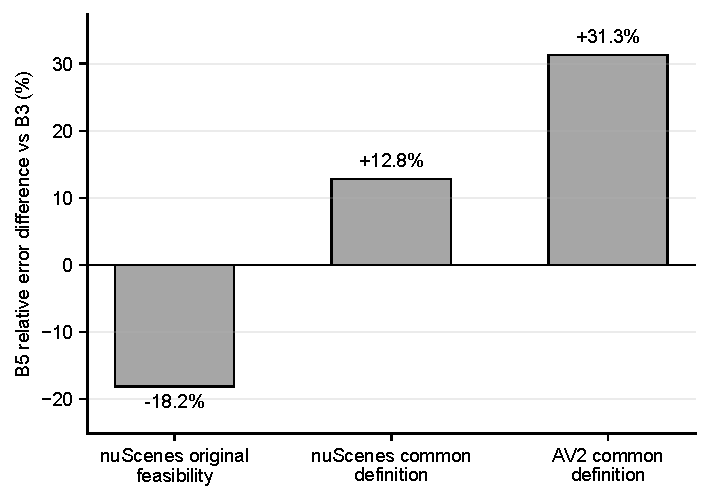
\includegraphics[width=0.98\columnwidth]{figure6_cross_dataset_reversal.pdf}
\caption{Cross-dataset harmonization at 500~ms with YOLO11n. Negative values favor B5; positive values favor B3.}
\label{fig:cross}
\end{figure}

Median per-object propagation times were 0.20--0.33~ms for B3/B5 across detectors; OC-SORT prediction took 0.22--0.24~ms. Association overhead, gate evaluation, and total pipelined overhead were not separately instrumented. The core leakage audit found no future-information flags in deployable predictions and no associations after the source timestamp. The provenance audit found no duplicate rows, incomplete T0--T6 sets, invalid coordinates, or detector/path mismatches; 49 headline recalculations agreed to a maximum absolute difference of $5\times10^{-14}$.

\section{Discussion}
The central finding of this study is that a physically motivated component---estimated object motion---consistently degraded a causal latency-compensation system when applied to every detection. The degradation appeared in two capacities of one detector family and in the architecturally distinct RT-DETR-L \cite{Zhao2024RTDETR}, so it cannot be attributed to the peculiarities of a single network. Nor can it be attributed to a weak reference: at the same frozen endpoint, ego-motion-only propagation also outperformed the causal predictions of SORT \cite{Bewley2016SORT}, ByteTrack \cite{Zhang2022ByteTrack}, and OC-SORT \cite{Cao2023OCSORT}, which represent the standard image-space treatment of exactly this extrapolation problem. The expectation inherited from pose-aware propagation---that modeling more of the true motion should reduce error \cite{Mahdian2024EMAP}---failed in a system where every component was fixed before the outcome was examined.

The component substitutions identify where the expectation breaks down. Let $d_o$ denote the true residual object displacement that remains after ego-motion correction, and let $\widehat{d}_o=d_o+\epsilon$ denote its causal estimate. Adding $\widehat{d}_o$ reduces error only when the image-space displacement induced by $\epsilon$ is smaller than the residual incurred by omitting $d_o$ altogether. Substituting oracle future displacement satisfied this condition and improved on B3 by 11.11\% and 9.85\% for the two YOLO detectors, which confirms that the residual signal exists and is worth recovering. The deployed estimator violated the same condition: velocity-sign flips and incorrect association together accounted for roughly 60\% of harmed objects, meaning the injected correction frequently pointed the wrong way rather than merely overshooting. Because constant-velocity extrapolation scales linearly with the horizon, this injected error also grew faster than the recoverable signal, from a 2.58\% penalty at 100~ms to 30.40\% at 500~ms. The underlying asymmetry is the one anticipated in Section~II: ego motion is measured once per frame from platform poses, whereas object motion must be estimated per object from noisy, intermittently associated detector history.

The full-frame evaluation fixes the boundary of this claim. B3 was superior on the localization-sensitive quantities---matched-object center error, IoU, AP75---and on recall and false-positive burden, but paired AP50:95 contrasts included zero for all three detectors, and no propagation-only method can produce an object that first appears during the latency interval. Ego-motion-only propagation is therefore the more reliable transport rule for boxes that already exist; it does not by itself address the broader streaming-perception problem of anticipating future frames \cite{Li2020Streaming,Yang2022Streaming,Wang2023ASAP}.

These results do not imply that object motion should never be modeled. In the exploratory strata, B5 outperformed B3 for objects within 20~m and for high-confidence detections---conditions in which lidar depth support is dense and association is comparatively unambiguous---while its disadvantage concentrated beyond 40~m and in the low-confidence stratum. Those observations delineate a plausible operating region, but they do not constitute a selection policy: the frozen causal gate, trained and thresholded before any extension outcome was seen, never selected B5 and therefore delivered no improvement over using B3 everywhere. The open problem is a selector that identifies trustworthy association and velocity estimates prospectively and survives validation on an untouched cohort; until such a selector exists, measured ego motion alone remains the defensible default.

Finally, the cross-dataset harmonization explains how the opposite conclusion was reached in the first place. The nuScenes feasibility analysis \cite{Caesar2020nuScenes} granted the object-motion estimator ground-truth instance-linked history and compared it against a weaker ego-motion baseline, and under those conditions B5 appeared 18.15\% better. Re-evaluating both datasets under common definitions---detector-derived history and the calibrated pose-based comparator---reversed the sign within nuScenes itself. Apparent benefit from a pipeline component can therefore originate in privileged information access or in comparator strength rather than in the component, and mechanistic credit should be assigned only after both are matched.

\subsection{Limitations}
The primary analysis used one forward camera and AV2 source-time lidar support, and does not evaluate end-to-end 3-D detection, learned future-frame detectors, or complete MOT metrics such as HOTA and identity switches. Ground-truth identities constructed evaluation pairs but were unavailable to deployable predictions. Forty of 50 held-out logs entered the high-yaw endpoint; the remainder lacked eligible matched comparisons. Mechanism diagnostics were available for the YOLO pipelines but not for RT-DETR-L, whose frozen pipeline did not emit all diagnostic fields. The causal-gate extension cohorts were incomplete and detector-imbalanced, with no RT-DETR prospective validation. Runtime instrumentation did not isolate association, gate, and end-to-end overhead. The beneficial near and high-confidence strata are exploratory and require external confirmation.

\balance
\section{Conclusion}
Across YOLO11n, YOLO11s, and RT-DETR-L, universal ego-plus-estimated-object-motion propagation worsened the frozen 300-ms high-yaw localization endpoint relative to ego-motion-only propagation, and B3 outperformed strong causal tracker predictions. Oracle substitutions showed that object motion is useful in principle, but association and velocity-estimation errors exceeded its correction signal. Full-frame results supported the localization conclusion for AP75, recall, and false positives; AP50:95 remained mixed. Nearby and high-confidence objects may define a selective operating region, but the frozen causal gate failed to identify it. For this system, measured ego motion is the defensible default; object-motion augmentation should be enabled only by a prospectively validated reliability criterion.

\section*{Data and Code Availability}
AV2 and nuScenes are publicly available under their respective licenses \cite{Wilson2021AV2,Caesar2020nuScenes}. Analysis code, frozen log lists, configuration files, aggregate tables, figure source data, and audit records will be released in a versioned repository and archived with a DOI before submission. Raw benchmark data and detector weights are not redistributed. [Insert repository release URL and archival DOI.]

\section*{Author Contributions}
Antonio Pereira Jr.: Conceptualization, methodology, formal analysis, software supervision, investigation, visualization, writing--original draft, and writing--review and editing. [Revise if additional authors are added.]

\section*{Conflict of Interest}
The author declares no competing interests.

\section*{Acknowledgment}
[Insert funding and institutional computing acknowledgments.]

\balance
\bibliographystyle{IEEEtran}
\bibliography{references}

\end{document}
